\section*{Chapter declaration}
\addcontentsline{toc}{section}{\numberline{}Chapter declaration}
The data, analysis, results, and discussion presented in this chapter were reported in my first-author publication ``ALMA reveals a compact and massive molecular outflow driven by the young AGN in a nearby ULIRG'' \citep{Holden2024}. The content of this chapter is based on that publication, which has been adapted into a suitable format for this thesis. The first stage of the ALMA CO(1--0) data reduction was performed by Tom Oosterloo, while all subsequent work is my own.

\newpage

\section{Introduction}
\label{section: alma_f13451_1232: introduction}

Another excellent object to investigate the impact and acceleration mechanism(s) of multiphase AGN-driven outflows is the ultraluminous infrared galaxy (ULIRG; $L_\mathrm{IR}$\;\textgreater\;$10^{12}$\;L$_\mathrm{\odot}$: \citealt{Sanders1996}) F13451+1232 --- also known as 4C12.50 --- which is a merger (\citealt{Gilmore1986, Heckman1986}) in a late pre-coalescence phase (nuclear separation $\sim$4.5\;kpc: \citealt{Tadhunter2018}). ULIRGs such as F13451+1232 are among the most rapidly evolving galaxies in the local universe due to merger-induced gas inflows feeding the central AGN and triggering star formation --- the exact situation modelled in some hydrodynamic simulations of galaxy evolution that include AGN-driven outflows as a feedback mechanism (e.g. \citealt{DiMatteo2005, Hopkins2008}). 

As a luminous radio source ($L_\mathrm{1.4\;GHz} = 1.9\times10^{26}$\;W\;Hz$^{-1}$), F13451+1232 contains radio emission on two distinct scales: small-scale emission within a radius of $\sim$130\;pc of the primary nucleus along position angle $\mathrm{PA}=151^\circ$ \citep{Stanghellini1997, Lister2003, Morganti2013_4c1250}, and larger-scale, diffuse emission extending to a radial distance of $\sim$77\;kpc from the primary nucleus along $\mathrm{PA}\sim180^\circ$ \citep{Stanghellini2005}. It has been proposed that this radio structure could be the result of two epochs of jet activity \citep{Stanghellini2005}, with the smaller-scale radio structure comprising a young, recently-restarted jet, and the larger-scale emission originating from a previous jet cycle. 

Because of the properties of its small-scale radio emission, F13451+1232 is also classified as a gigahertz-peaked-spectrum (GPS) source (see Section\;\ref{section: introduction: outflows: taxonomy_of_agn: css_and_gps_sources}, and \citealt{ODea2021} for a review); such sources are associated with powerful jet-ISM interactions that may accelerate gas outflows in multiple phases \citep{Mukherjee2016, Holt2006, Santoro2018, Santoro2020, Kukreti2023}. In addition, given the object's high optical-emission-line luminosity ($L_\mathrm{[OIII]}=1.45\times10^{43}$\;erg\;s$^{-1}$: \citealt{Rose2018}) --- leading to its additional classification as a type-2 quasar (QSO2)\footnote{F13451+1232 is included in the QUADROS sample of ULIRGs \citep{Rose2018}, and the QSOFEED sample of type-2 quasars \citep{RamosAlmeida2022}.} --- it might also be expected to accelerate prominent outflows via radiation pressure. Therefore, F13451+1232 is ideal for investigating the properties and acceleration mechanisms of multi-phase outflows in an object that is considerably more luminous at optical and radio wavelengths than the Seyfert galaxies studied in Chapters\;\ref{chapter: xshooter_ic5063} and \ref{chapter: stis_seyferts}.

Despite the fact that outflows in F13451+1232 have been confirmed in the coronal \citep{VillarMartin2023}, warm ionised \citep{Holt2003, Holt2011, Rose2018, VillarMartin2023}, and neutral atomic (HI + NaID: \citealt{Morganti2005, Rupke2005, Morganti2013_4c1250}) gas phases, there has so far not been a robust detection of molecular outflows in this object (\citealt{Fotopoulou2019, Lamperti2022}; see discussion in \citealt{VillarMartin2023}). In nearby AGN where molecular outflows have been detected, it is often found that they contain more mass and kinetic power than the warmer phases (e.g. Chapters \ref{chapter: xshooter_ic5063} and \ref{chapter: stis_seyferts}; \citealt{Fiore2017, RamosAlmeida2019, Speranza2024}). In this context, it is important to note that the warm-ionised and neutral-atomic outflows in F13451+1232 have relatively modest mass outflow rates ($\sim$6--$12$\;M$_\odot$\;yr$^{-1}$: \citealt{Morganti2013_4c1250, Rose2018}); therefore, if molecular outflows are present, they could potentially carry enough mass to change the interpretation of AGN feedback in this important object. 

Models of galaxy evolution predict that AGN triggered at the peaks of mergers (such as F13451+1232) launch prominent, galaxy-wide ($r$\;\textgreater\;5\;kpc) outflows (e.g. \citealt{Springel2005, Hopkins2008, Johansson2009}). However, a cold-molecular outflow in a similar source, PKS 1549-79, was found to be compact ($r$\;\textless\;120\;pc: \citealt{Oosterloo2019}), as were the previously-detected neutral HI ($r_\mathrm{HI}$\;\textless\;100\;pc: \citealt{Morganti2013_4c1250}) and warm-ionised ($r_\mathrm{[OIII]}\sim69$\;pc: \citealt{Tadhunter2018}) outflows in F13451+1232. In order to complete the multi-phase information for this important object, and to directly determine if the spatial extents of any cold-molecular outflows are consistent with the predictions of models of galaxy evolution, here I present high-spatial resolution ($0.113\times0.091$\;arcsecond or $247\times119$\;pc beam size), high-sensitivity Atacama Large Millimeter/submillimeter Array (ALMA) CO(1--0) observations of the inner few kiloparsecs of the primary nucleus of F13451+1232.

Throughout this chapter, I assume a cosmology of $H_0=70$\;km\;s$^{-1}$\;Mpc$^{-1}$, $\Omega_\mathrm{m}=0.3$, and $\Omega_\mathrm{\lambda}=0.7$. This corresponds\footnote{Calculated using Ned Wright's Javascript Cosmology Calculator \citep{Wright2006}.} to an arcsecond-to-kpc spatial conversion factor of 2.189\;kpc/arcsec and a luminosity distance of $D_\mathrm{L}=570$\;Mpc at the redshift of F13451+1232 ($z=0.121680$: \citealt{Lamperti2022}).

\section{Observations and data reduction}
\label{section: alma_f13451_1232: observations_and_data_reduction}

F13451+1232 was observed in Band 3 of ALMA on two nights using two different configurations of the 12\;m array (Project Code 2019.1.01757.S): the array configuration used on the 10th September 2021 (baselines $=180$--16200\;m) resulted in a beam size of $0.083\times0.069$\;arcseconds, while the configuration used on the 28th September 2021  (baselines $=70$--14400\;m) resulted in a beam size of 0.166$\times$0.123\;arcseconds. The total time on-source was 5588\;seconds ($\sim$1.5\;hours). Four spectral windows were used for the observations: one centred on 102.790\;GHz with a bandwidth of 1.875\;GHz (covering the CO(1--0) line), and the remaining three centred on 104.581\;GHz, 90.977\;GHz, and 92.477\;GHz with bandwidths of 2.000\;GHz (covering the continuum). J1337-1257 and J1353+1435 were observed to provide bandpass/flux and phase calibration, respectively; phase self-calibration was performed using the \textsc{Miriad} data reduction package \citep{Sault1995}.

The CO(1--0) transition was targeted for two reasons. First, the ALMA observing band that covers the CO(1--0) line is wider than those that cover higher-order transitions such as CO(2--1) or CO(3--2), and therefore facilitates more accurate continuum subtraction. Second, the CO(1--0) transition is less susceptible to gas excitation conditions than the higher-order CO transitions, and hence may be a more reliable probe of molecular gas masses in ULIRGs.

In order to check for instrumental errors such as bandpass and spectral-calibration issues, three CO(1--0) line datacubes were produced: two using the visibilities of the two different array configurations separately, and one produced by combining the visibilities from both observation sets (with a final beam size of $0.113\times0.091$\;arcseconds, $\mathrm{PA}=-51.8^\circ$). To optimise the column-density sensitivity, and to ensure that the dirty beam was not significantly non-Gaussian, each CO(1--0) line cube was made using Briggs weighting with \mbox{robust $=1$}. When inspecting these cubes individually, no indications of bandpass or spectral-calibration issues were found.

The data products produced by the automated ALMA pipeline are potentially affected by issues related to continuum subtraction, which are a consequence of the bright and steep continuum emission produced by the primary nucleus of F13451+1232. Therefore, for all three datacubes, the respective visibilities (as calibrated by the ALMA pipeline) were used as an initial step, to which standard self-calibration (using continuum images made from the line-free channels) was applied. Line datacubes were then created, and the continuum in each was removed by subtracting a linear function that was fitted to the continuum on either side of (but excluding) the CO(1--0) emission. A continuum image was also generated from the combined visibilities of both observations using the continuum spectral windows. Least-squares fitting was performed using the \textsc{AstroPy} \citep{AstropyCollaboration2013, AstropyCollaboration2018} \textsc{Python} module to fit a two-dimensional Gaussian profile to the point source in this continuum image; the centroid position (13:47:33.36 +12 17 24.23) was taken to be the location of the nucleus. The continuum image was made using uniform weighting and has a resolution of $0.049\times0.033$\;arcseconds ($\mathrm{PA}=-46.8^\circ$).

To ensure the highest sensitivity and signal-to-noise, only the combined CO(1--0) datacube is considered in the main analysis of this chapter; this cube has a root-mean-square (RMS) noise of $0.148$\;mJy\;beam$^{-1}$ for a velocity resolution of 28.8\;km\;s$^{-1}$.

\newpage

\section{Analysis and results}
\label{section: alma_f13451_1232: analysis_and_results}

\subsection{Moment maps}
\label{section: alma_f13451_1232: analysis_and_results: moment_maps}

\begin{figure*}[!t]
    \centering
    \begin{subfigure}[]{\linewidth}
        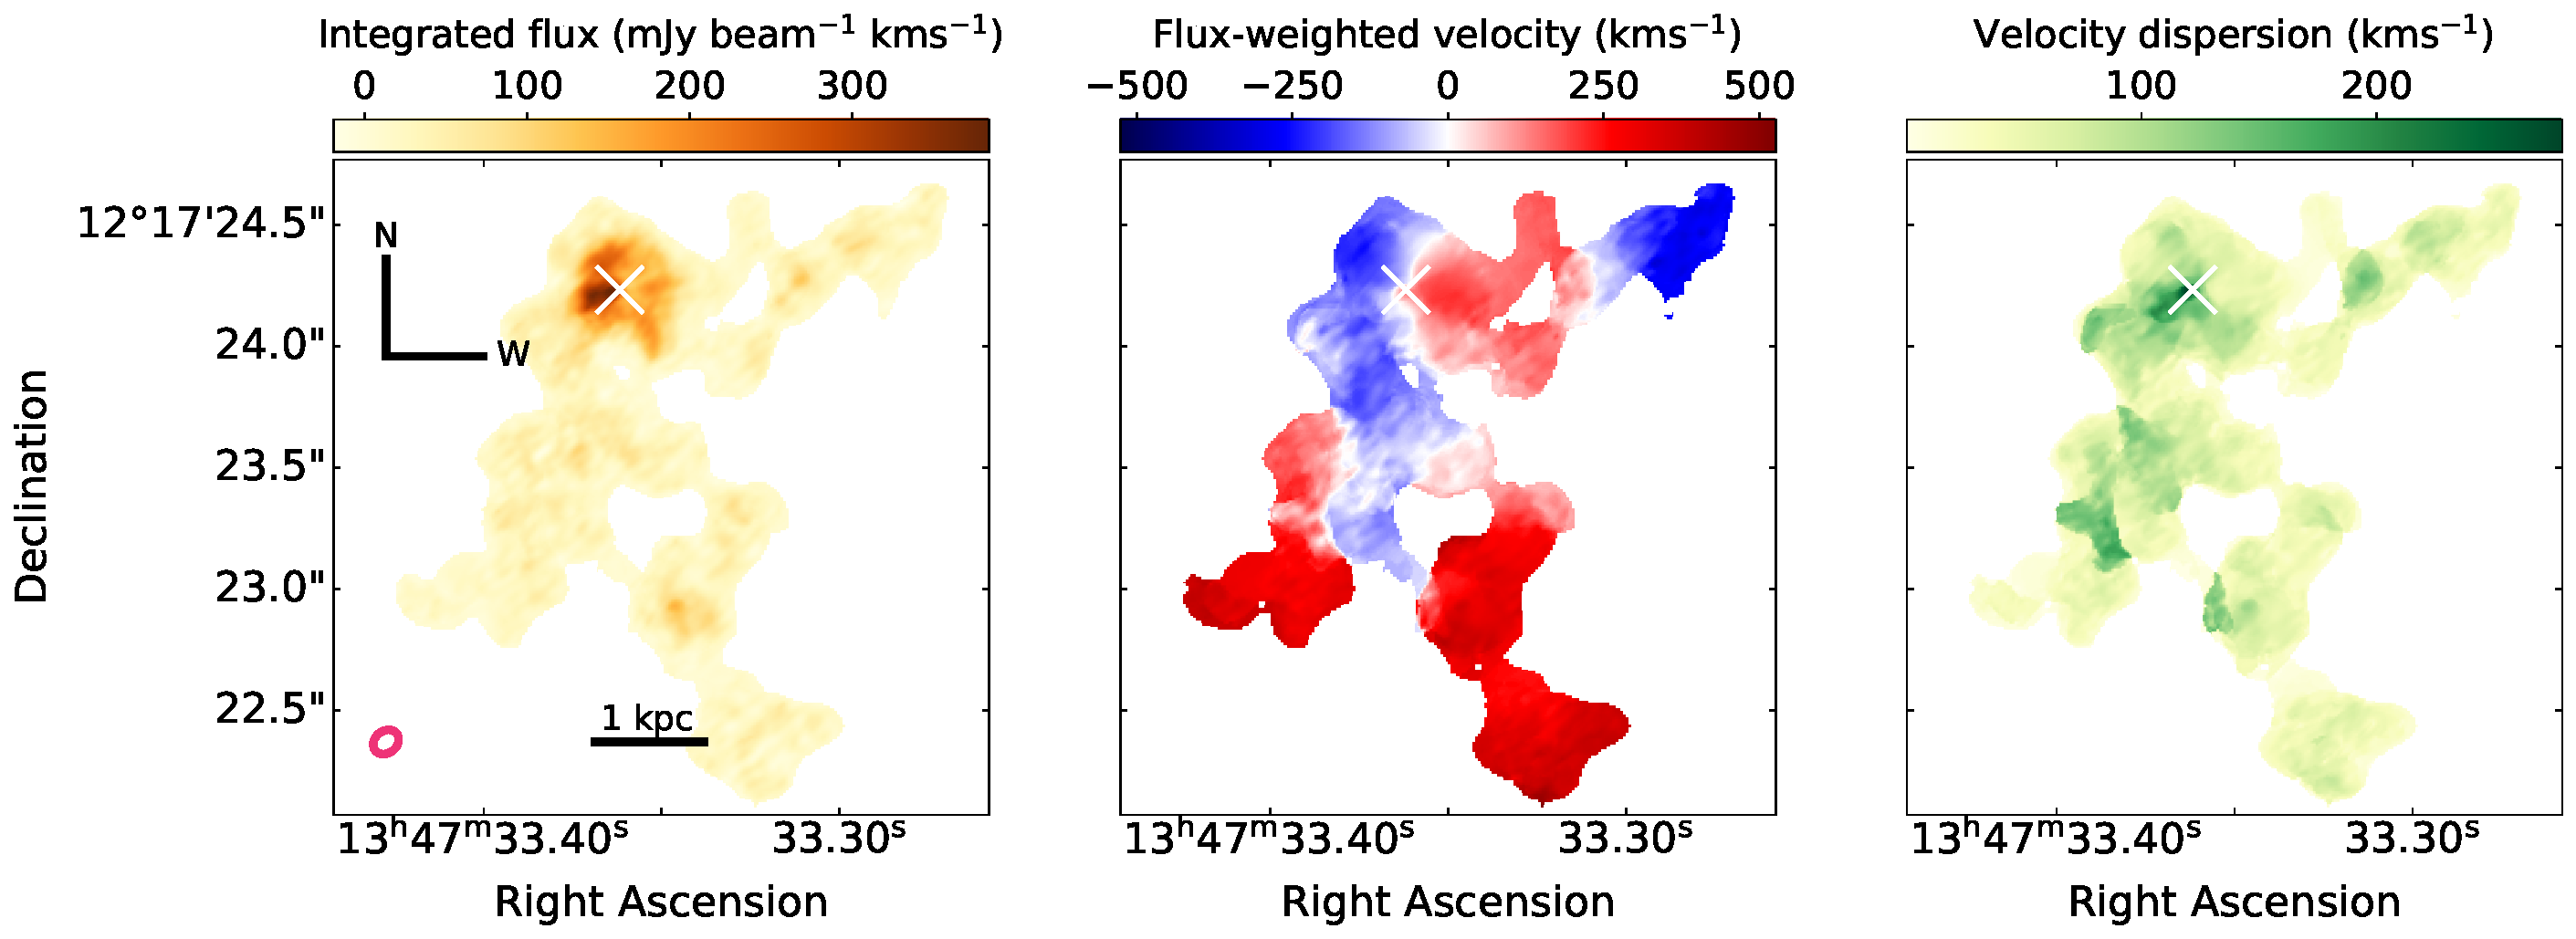
\includegraphics[width=1\linewidth, trim={0 1.5cm 0 0}, clip]{figures/alma_f13451_1232/large_fov_moment_maps.pdf}
    \end{subfigure} \\
    \vspace*{\baselineskip}
    \begin{subfigure}[]{\linewidth}
        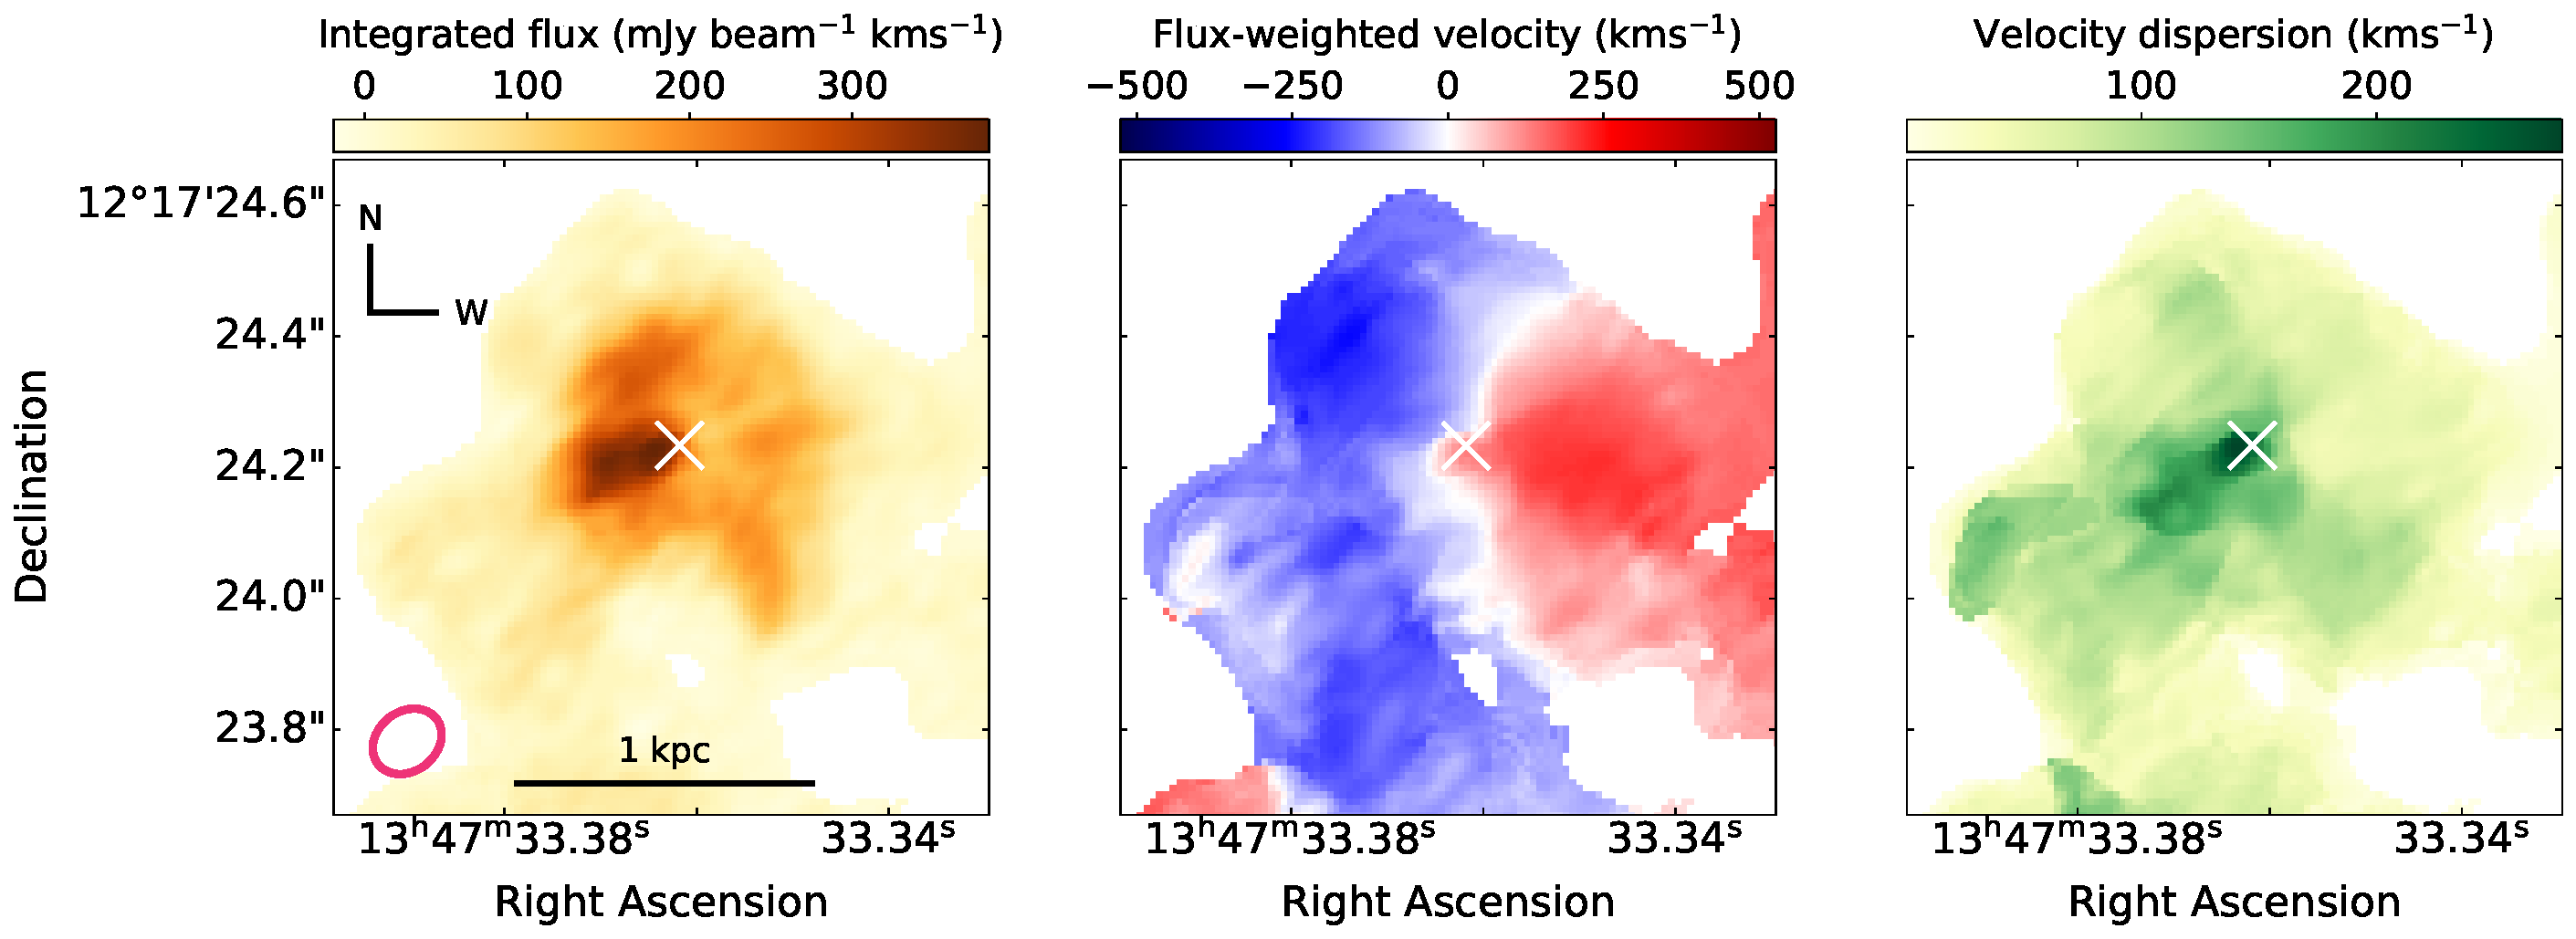
\includegraphics[width=1\linewidth, trim={0 0 0 2.93cm}, clip]{figures/alma_f13451_1232/moment_maps.pdf}
    \end{subfigure}
    \caption[Moment 0, 1, and 2 maps for the central kiloparsecs of the primary nucleus of F13451+1232.]{Integrated flux (moment 0; left panels), flux-weighted velocity (moment 1; middle panels), and velocity dispersion (moment 2; right panels) maps for the central $6\times6$\;kiloparsec (top panels) and inner-kiloparsec region (bottom panels) of the primary nucleus of F13451+1232. The white cross marks the continuum centre, which is taken to be the position of the AGN nucleus. The beam size of the observations is shown as a pink ellipse in the bottom left corner, and a 1\;kpc scale bar is shown in black.}
    \label{fig: alma_f13451_1232: moment_maps}
\end{figure*}

To investigate the flux and kinematic structures of the CO(1--0) emission around the primary nucleus of F13451+1232, moment maps of the combined datacube were created using the \textsc{SoFiA-2} source-finding pipeline \citep{Serra2015, Serra2021}. \textbf{In order to ensure that only genuine emission over a range of spatial scales (and of varying surface brightness) was used when producing the moment maps}, \textsc{SoFiA-2} first applied different combinations of spatial and velocity smoothing to the datacube: Gaussian filters with FWHMs of 0, 3, 6, 12, and 15 pixels were used for the spatial smoothing, and boxcar filters of widths 0, 3, 7, and 15 channels were used for the velocity smoothing. For each combination of spatial and velocity smoothing, emission above $4\sigma_\mathrm{rms}$ \textsc{(measured from the original cube in a region that did not contain emission)} was added to a total mask. This mask was then applied to the original, non-smoothed datacube, from which the maps in Figure\;\ref{fig: alma_f13451_1232: moment_maps} were produced. 

In the $6\times6$\;kpc moment maps (upper panels of Figure\;\ref{fig: alma_f13451_1232: moment_maps}), cold-molecular gas is detected to radial distances of $\sim$2.5\;arcseconds ($\sim$5.5\;kpc) south of the primary nucleus, and $\sim$1\;arcsecond ($\sim$2\;kpc) to the west. This large-scale ($r$\;\textgreater\;1\;kpc) emission, which has velocities in redshift and blueshift of up to $|v|\sim500$\;km\;s$^{-1}$, is indicative of gas that has been disturbed by the merger.

Within the central kiloparsec of the primary nucleus (Figure\;\ref{fig: alma_f13451_1232: moment_maps}), there is clear evidence for a disk with radius $r_\mathrm{disk}\sim0.5$\;kpc centred on the nucleus, blueshifted to the east and redshifted to the west, with a projected maximum flux-weighted velocity of 200--250\;km\;s$^{-1}$. In addition, there is an extended region (up to $r\sim0.3$\;arcseconds or 660\;pc from the nucleus along $\mathrm{PA}=120^\circ$) of emission with higher velocity dispersions ($\sigma$\;\textgreater\;150\;km\;s$^{-1}$) than that of the disk. Furthermore, a particularly prominent redshifted component with a velocity dispersion of $\sim$250\;km\;s$^{-1}$ is seen within a radius of $r\sim0.1$\;arcseconds ($r\sim220$\;pc) of the continuum centre.


\subsection{BBarolo modelling of the gas disk}
\label{section: alma_f13451_1232: analysis_and_results: disk}


To separate non-gravitational kinematics from those expected from a rotating gas disk, the disk was modelled using the \textsc{3DFIT} task from the \textsc{BBarolo} tool \citep{DiTeodoro2015}. The \textsc{3DFIT} task fits a series of concentric rings to the data in three spatial dimensions and three velocity dimensions (the rotational velocity, $v_\mathrm{rot}$; the radial velocity, $v_\mathrm{rad}$, and the velocity dispersion $v_\mathrm{disp}$).

The fitting procedure followed the methodology outlined in \citet{AlonsoHerrero2018}, \citet{DominguezFernandez2020}, and \citet{RamosAlmeida2022}. Throughout, the centre of the disk model was fixed to be the position of the continuum centre (as measured from a two-dimensional Gaussian fit to the continuum image: Section\;\ref{section: alma_f13451_1232: observations_and_data_reduction}). An initial fit was first performed using the \textsc{3DFIT} task in which the radial velocities of the rings were fixed to be 0\;km\;s$^{-1}$ and the scale height of the disk ($z_\mathrm{0}$) was fixed to 0\;pc. The remaining parameters were allowed to vary; initial values for the rotational velocity and velocity dispersion were based on the flux-weighted velocity shift and velocity dispersion maps (Figure\;\ref{fig: alma_f13451_1232: moment_maps}), the initial value of the inclination ($i_\mathrm{initial}=38^\circ$) was based on the measured ratio of the projected disk major and minor axes while assuming a circular disk, and the initial value for the PA was set to that previously estimated from two-dimensional spectroastrometry of CO(2--1) observations of the disk by \citet{Lamperti2022}. However, limits were imposed on the variation of these free parameters --- between successive rings, the rotational velocity was not allowed to change by more than $\pm$50\;km\;s$^{-1}$, nor were the inclination and PA allowed to change by more than $\pm20^\circ$. The fits used uniform weighting and local normalisation. It should be noted that, since the physical size of the modelled rings is much less than the beam size of the observations, the properties of adjacent rings are correlated. However, this does not have a significant effect on the maximum rotational velocity of the disk model (nor does changing the values of the initial parameters), and therefore does not affect the interpretations made in this analysis.

\begin{figure*}[!p]
    \centering
    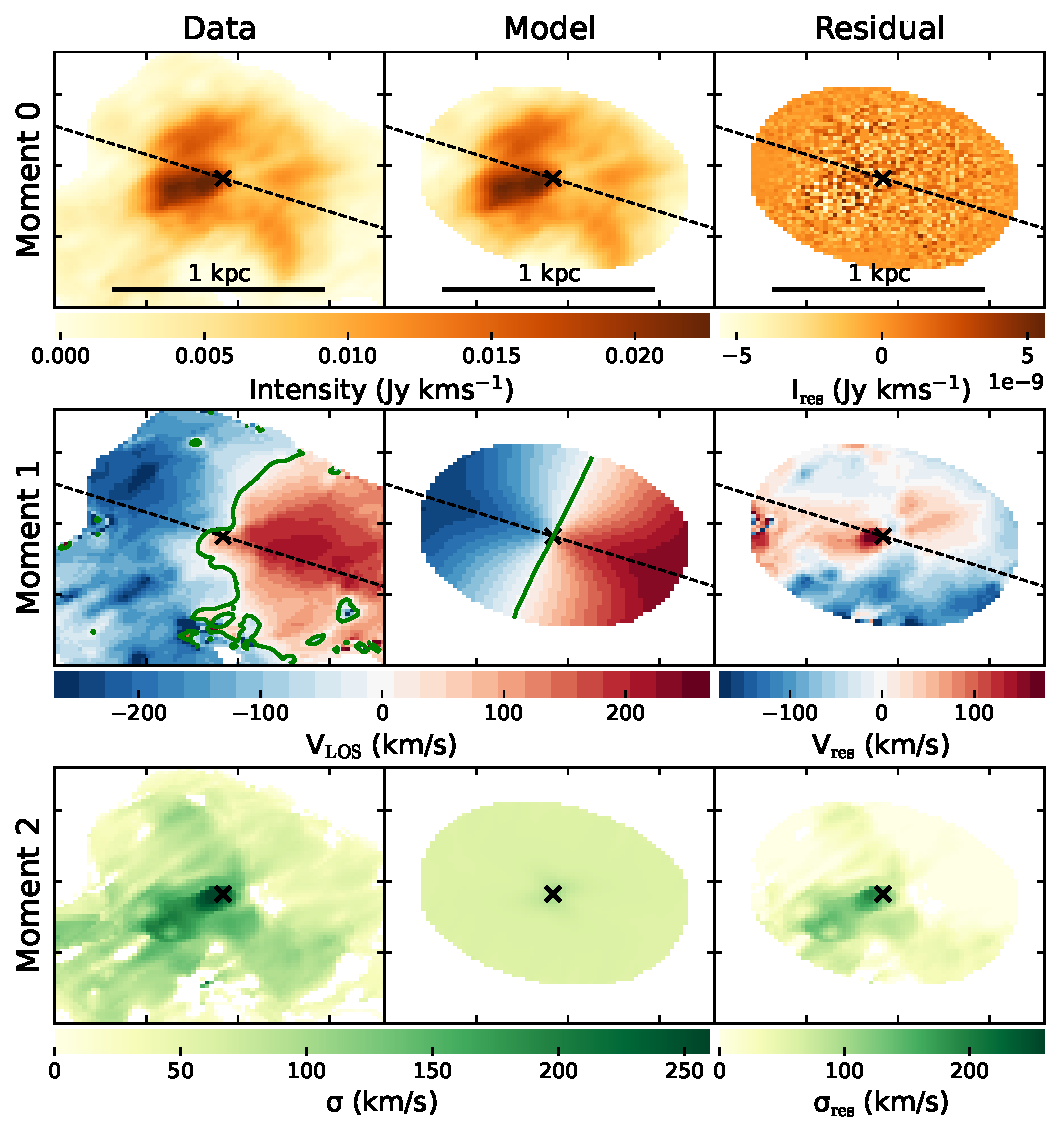
\includegraphics[width=\linewidth]{figures/alma_f13451_1232/disk_moment_maps.pdf}
    \caption[Moment 0, 1, and 2 maps (and residuals = data - model) for the \textsc{BBarolo 3DFit} model of the kiloparsec-scale disk in the primary nucleus of F13451+1232.]{Integrated flux (moment 0; top), flux-weighted velocity (moment 1; middle), and velocity dispersion (moment 2; bottom) maps of the CO(1--0) data (left), the \textsc{BBarolo} disk model (middle), and residuals (data - model; right). The ticks have separations of 0.2\;arcseconds. The black dashed line shows the PA of the modelled disk, whereas the black cross shows the disk centre (which was set to be the continuum centre position; see Section\;\ref{section: alma_f13451_1232: observations_and_data_reduction}). The green lines in the middle-row panels are isovelocity contours at 0\;km\;s$^{-1}$.}
    \label{fig: alma_f13451_1232: bbarolo_model}
\end{figure*}


In order to ensure that the overall radial extent and kinematics of the disk were accurate --- and to alleviate potential problems with fit degeneracy arising from having a high number of free parameters --- the results of the initial fit were used as a basis for a second fit. For this second run, I fixed the velocity dispersion, inclination, and PA to the values determined from the first run, so that only the rotational velocity was allowed to vary. The final model parameters for each ring are presented in Table\;\ref{tab: bbarolo_model}; Figure\;\ref{fig: alma_f13451_1232: bbarolo_model} presents the moment maps and residuals of the final disk model. High flux-weighted velocities ($V_\mathrm{LOS}$\;\textgreater\;200\;km\;s$^{-1}$) and velocity dispersions ($\sigma\sim200$\;km\;s$^{-1}$) due to non-rotational kinematics can be seen in the residual maps near the centre of the disk.

In the final \textsc{BBarolo} model, the disk has an average inclination of $i\approx54^\circ$ (where $i=0^\circ$ corresponds to the disk being face-on), and its major axis lies along $\mathrm{PA}\approx248^\circ$; the deprojected rotational velocity increases from $v_\mathrm{rot}=246$\;km\;s$^{-1}$ to $v_\mathrm{rot}=307$\;km\;s$^{-1}$ over the radius range 28\;pc\;\textless\;$r_\mathrm{disk}$\;\textless\;560\;pc. I highlight that the purpose of this modelling was solely to give a reasonable estimate of the maximum rotational velocity of the molecular gas, which is needed to robustly identify non-rotational motions. Considering this, it is notable that the high-velocity-dispersion emission ($\sigma$\;\textgreater\;150\;km\;s$^{-1}$) seen near the disk in the moment maps (Figure\;\ref{fig: alma_f13451_1232: moment_maps}) cannot be accounted for by the \textsc{BBarolo} model (see Figure\;\ref{fig: alma_f13451_1232: bbarolo_model}), and thus cannot be explained as being part of the rotating gas disk. 


\begin{table*}[!t]
    \centering
    \renewcommand{\arraystretch}{1.2}
    \begin{tabular}{cccccc}
    $r_\mathrm{ring}$\;(arcseconds) & $r_\mathrm{ring}$\;(pc) & $v_\mathrm{rot}$\;(km\;s$^{-1}$) & $v_\mathrm{disp}$\;(km\;s$^{-1}$) & $i$\;$(^\circ)$  & PA\;$(^\circ)$ \\ \hline
    0.013     & 29    & 248    & 5.5      & 62.2   & 242   \\
    0.040     & 88    & 250    & 24.6     & 58.6   & 236   \\
    0.067     & 147    & 212    & 91.1     & 55.9   & 236   \\
    0.094     & 206    & 249    & 72.5     & 53.8   & 240   \\
    0.121     & 265    & 268    & 65.8     & 52.4   & 245   \\
    0.148     & 324    & 281    & 62.8     & 51.4   & 252   \\
    0.175     & 383    & 293    & 61.2     & 50.8   & 258   \\
    0.202     & 442    & 312    & 68.3     & 50.5   & 261   \\
    0.229     & 501    & 301    & 61.5     & 50.3   & 259   \\
    0.256     & 560    & 314    & 58.3     & 50.1   & 252  
    \end{tabular}
    \caption[Parameters of the \textsc{BBarolo 3DFit} model of the kiloparsec-scale disk in the primary nucleus of F13451+1232.]{Final parameters for each ring of the \textsc{BBarolo 3DFit} disk model. The distance of each ring to the fixed disk centre ($r_\mathrm{ring}$) is given in both arcseconds and parsecs. Here, $v_\mathrm{rot}$ and $v_\mathrm{disp}$ are the rotational velocities and velocity dispersions of each ring, respectively.}
    \label{tab: bbarolo_model}
\end{table*}


\subsection{Kinematics of the non-rotating gas}
\label{section: alma_f13451_1232: analysis_and_results: outflow_kinematics}

To investigate the non-rotational kinematics further, I binned the velocity channels of the original cube by a factor of three and applied Hanning smoothing using the \textsc{CASA} software suite \citep{Bean2022} to improve the signal-to-noise ratio of the emission. This resulted in a cube of velocity resolution 86.4\;km\;s$^{-1}$ and an RMS noise of $0.083$\;mJy\;beam$^{-1}$. Using the \textsc{pvextractor Python} module\footnote{\url{https://pvextractor.readthedocs.io/en/latest/}}, $1.00\times0.05$\;arcsecond slices, centred on the nucleus, were extracted from both this datacube and the \textsc{BBarolo} disk-model datacube along the major axis of the disk ($\mathrm{PA}=248^\circ$) and in the direction of the high-velocity-dispersion gas near the nucleus ($\mathrm{PA}=120^\circ$). From these slices, position-velocity (PV) diagrams were produced, which are presented in Figure\;\ref{fig: alma_f13451_1232: pv_diagrams}. In the PV diagrams, there is clear evidence for non-rotational kinematics, with detected velocities being well above the projected maximum rotational disk velocity given by the \textsc{BBarolo} model. There is intermediate-velocity emission (300\;\textless\;$|v|$\;\textless\;400\;km\;s$^{-1}$) seen in both blueshift and redshift along $\mathrm{PA}=120^\circ$, in the ranges 0.1\;\textless\;$r$\;\textless\;0.3\;arcseconds and 0.0\;\textless\;$r$\;\textless\;0.2\;arcseconds, respectively, to the southeast (SE) of the nucleus. Moreover, the compact ($r$\;\textless\;0.1\;arcseconds) redshifted feature visible in the moment maps (Figure\;\ref{fig: alma_f13451_1232: moment_maps}) can be seen in the PV diagrams between 400\;\textless\;$v$\;\textless\;680\;km\;s$^{-1}$, located close to the nucleus.

\begin{figure*}[!p]
    \centering
    \begin{subfigure}[b]{0.75\textwidth}
        \centering
        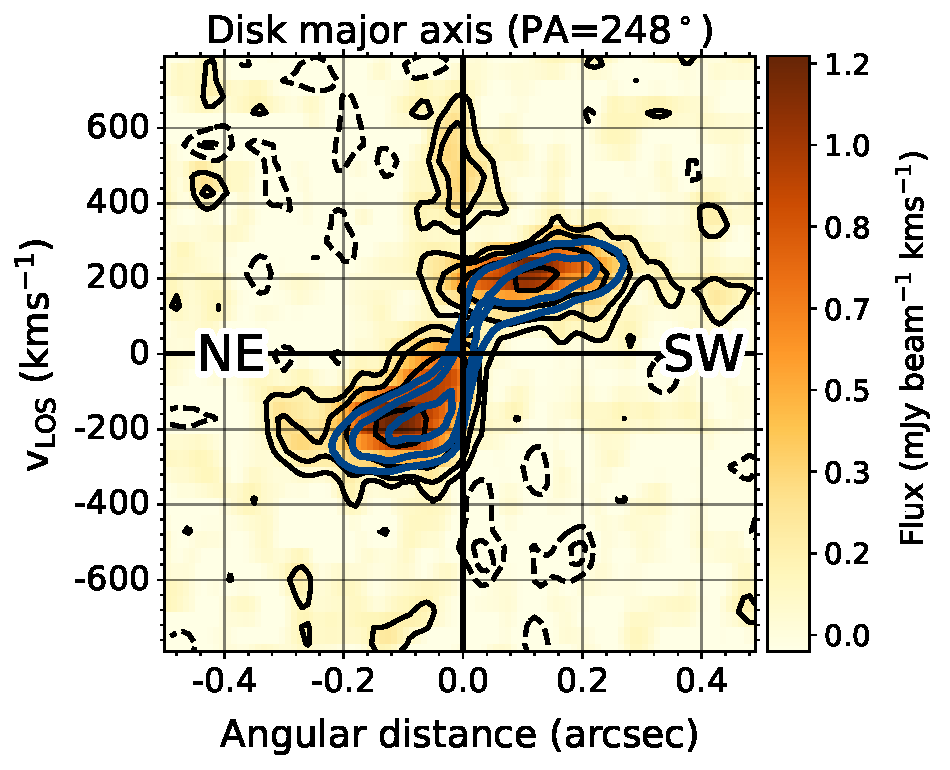
\includegraphics[width=\textwidth]{figures/alma_f13451_1232/pv_248deg.pdf}
    \end{subfigure}
    \hspace{1em}
    \begin{subfigure}[b]{0.75\textwidth}
        \centering
        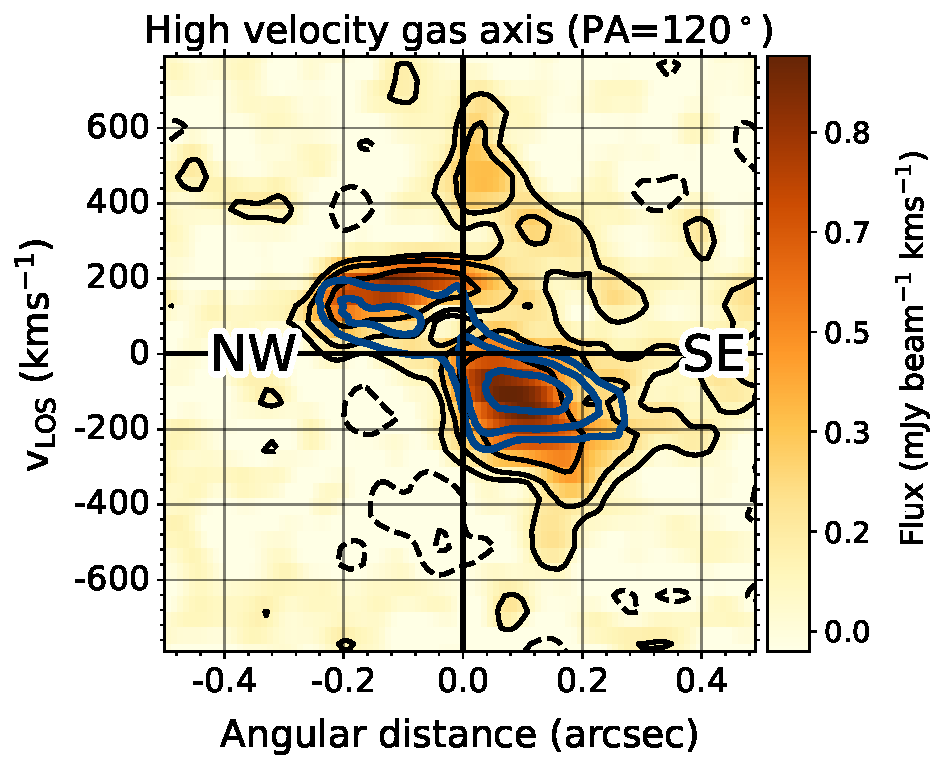
\includegraphics[width=\textwidth]{figures/alma_f13451_1232/pv_120deg.pdf}
    \end{subfigure}
    \caption[CO(1--0) position-velocity (PV) diagrams for $1.00\times0.05$\;arcsecond slices with $\mathrm{PA}=248^\circ$ and $\mathrm{PA}=120^\circ$, centred on the primary nucleus of F13451+1232.]{Position-velocity (PV) diagrams for $1.00\times0.05$\;arcsecond slices with $\mathrm{PA}=248^\circ$ (upper panel; the major axis of the disk) and $\mathrm{PA}=120^\circ$ (lower panel; the direction of the high-velocity-dispersion emission seen in Figure\;\ref{fig: alma_f13451_1232: moment_maps}), centred on the continuum centre. CO(1--0) emission is shown in yellow/orange, with black contours at the $-3\sigma_\mathrm{rms}$, $-1.5\sigma_\mathrm{rms}$, 1.5$\sigma_\mathrm{rms}$, 3$\sigma_\mathrm{rms}$, 6$\sigma_\mathrm{rms}$, and 12$\sigma_\mathrm{rms}$ levels (dashed: negative; solid: positive); solid blue contours show the flux from the \textsc{BBarolo} disk model at the same $\sigma_\mathrm{rms}$ levels. Extended, intermediate-velocity emission is seen in both redshift and blueshift in the $\mathrm{PA}=120^\circ$ diagram, and a compact, higher-velocity feature (400\;\textless\;$v$\;\textless\;680\;km\;s$^{-1}$) centred approximately on the nucleus (0.0\;arcsec) can clearly be seen in both diagrams.}
    \label{fig: alma_f13451_1232: pv_diagrams}
\end{figure*}

\begin{figure}[!h]
    \centering
    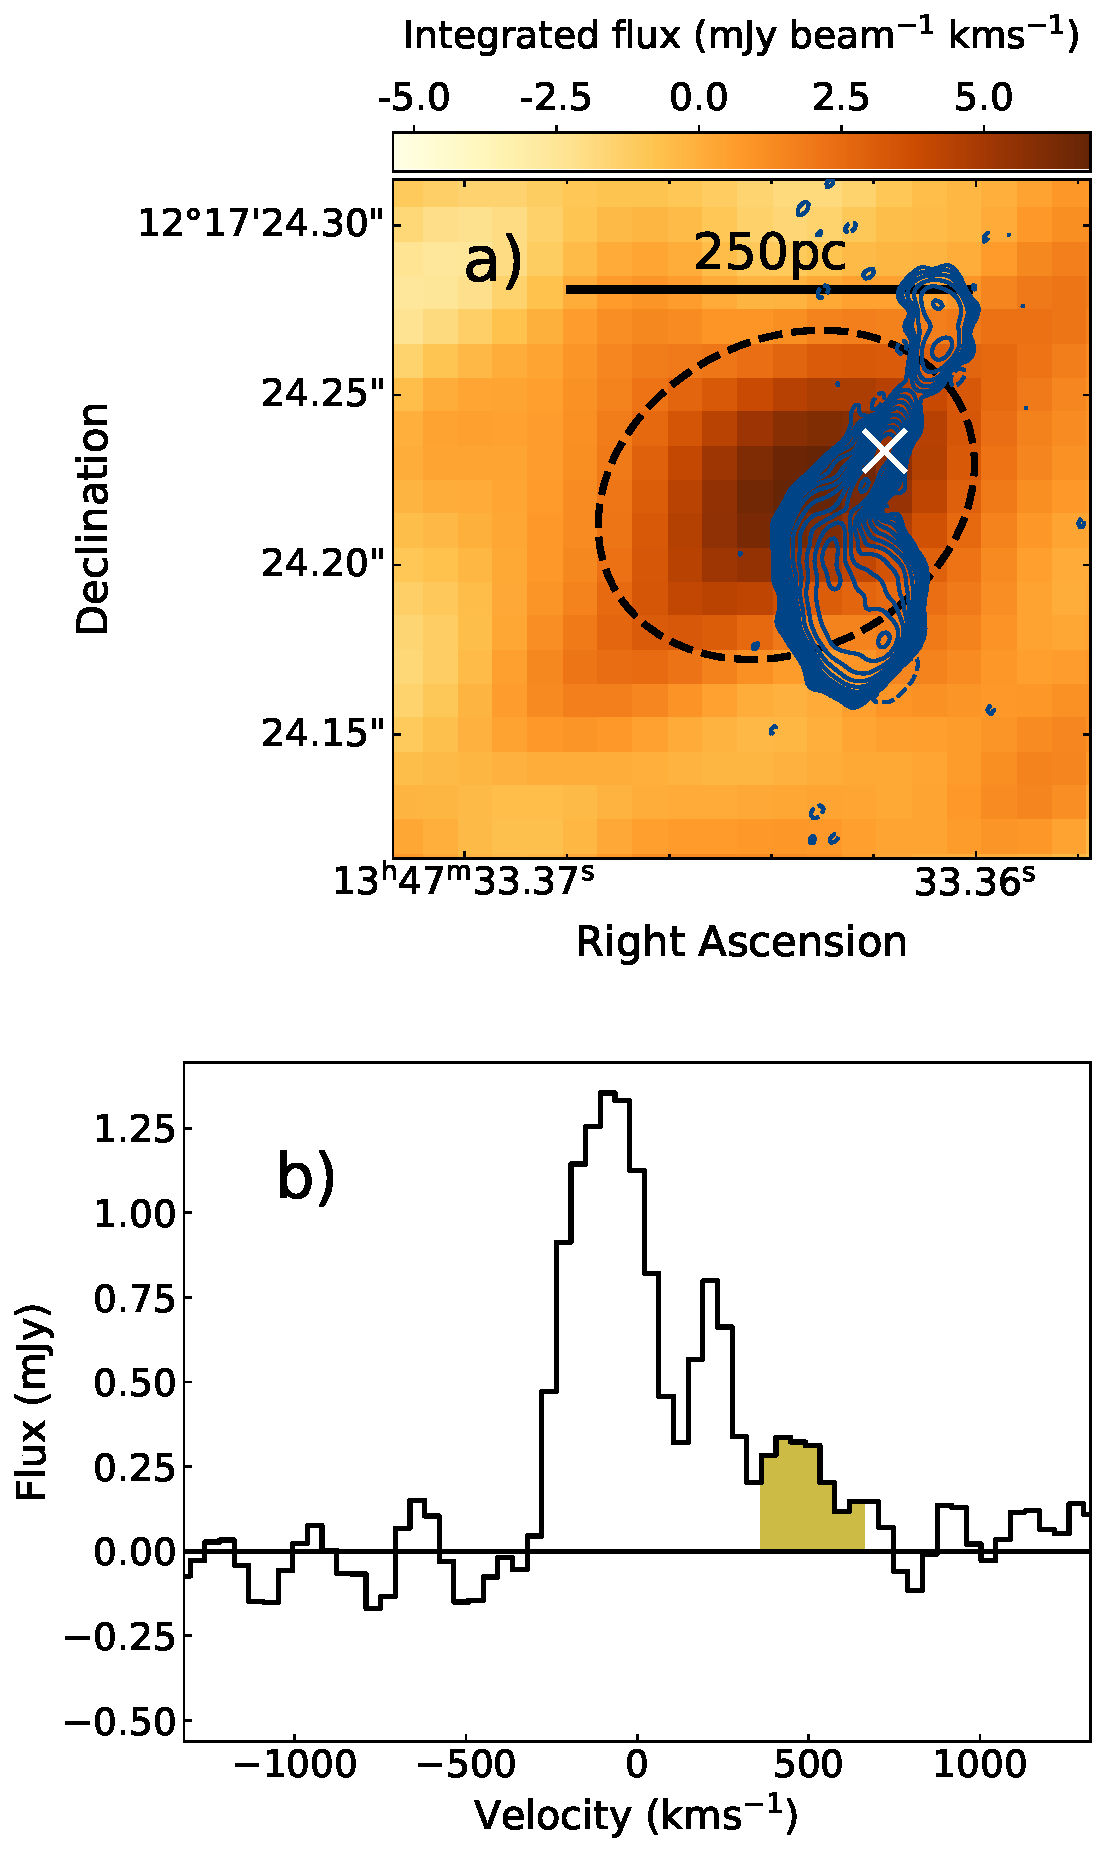
\includegraphics[width=0.65\linewidth]{figures/alma_f13451_1232/outflow_moment_map.pdf}
    \caption[\textbf{a)} Integrated CO(1--0) flux map of the nuclear outflow in F13451+1232, with VLBI 1266\;MHz continuum imaging from \citet{Morganti2013_4c1250} showing the small-scale radio structure; \textbf{b)} CO(1--0) velocity profile of the nuclear outflow.]{\textbf{a)} Integrated flux map (orange--brown) of the velocity channels between 400\;\textless\;$v$\;\textless\;680\;km\;s$^{-1}$. The dashed black ellipse shows the aperture extracted from the datacube to derive the mass of the outflow; the corresponding line profile is shown in Figure\;\ref{fig: alma_f13451_1232: outflow_moment_map}b. The small-scale radio structure, as seen in VLBI 1266\;MHz continuum imaging \citep{Morganti2013_4c1250}, is shown as dark blue solid contours at the $0.3\times$($-1$, 1, 2, 4, 8, 16, 32, 64, 128, 256, 512, 1024) mJy/beam levels, whereas the white cross marks the position of the continuum centre seen in the ALMA CO(1--0) observations (Section\;\ref{section: alma_f13451_1232: observations_and_data_reduction}). \textbf{b)}\;CO(1--0) line profile extracted from the aperture that covers the outflow; the line profile shown was extracted from the 84\;km\;s$^{-1}$ velocity resolution combined datacube. The part of the line profile that is taken to represent outflowing gas (400\;\textless\;$v$\;\textless\;680\;km\;s$^{-1}$) is shaded in yellow.}
    \label{fig: alma_f13451_1232: outflow_moment_map}
\end{figure}

\subsection{Comparison to the small-scale radio structure}
\label{section: alma_f13451_1232: analysis_and_results: radio_structure}

Due to the velocities at which the compact, high-velocity nuclear feature is detected, it is unambiguously distinct from the rotating gas disk: it may be interpreted as either an inflow moving towards the nucleus on the observer's side of the disk, or an outflow originating from the nucleus on the far side of the disk. Spatial comparison of the high-velocity flow to the small-scale radio structure may provide an indication of the nature of this flowing gas and, if it is an outflow, the driving mechanism. Figure\;\ref{fig: alma_f13451_1232: outflow_moment_map}a shows the flux map integrated over the range 400\;\textless\;$v$\;\textless\;680\;km\;s$^{-1}$ --- in which peak emission is detected above the 6$\sigma_\mathrm{rms}$ level --- along with VLBI 1266\;MHz continuum imaging (from global VLBI experiment GM62B; data presented and detailed in \citealt{Morganti2013_4c1250}) of the central $0.20\times0.20$\;arcseconds ($440\times440$\;parsecs). The beam size of the VLBI observations was $8.01\times4.89$\;milliarcseconds ($\mathrm{PA}=-20.2^\circ$). Due to the small uncertainties in the ALMA pointing, the VLBI image was offset from the continuum centre by $\sim$0.1\;arcseconds; this pointing error was corrected for by aligning the compact core seen in the VLBI image with the continuum centre, as it is expected that the same source is being imaged at different spatial resolutions. 

By fitting a two-dimensional Gaussian profile to the integrated high-velocity CO(1--0) emission in Figure\;\ref{fig: alma_f13451_1232: outflow_moment_map}a using the \textsc{emcee} Python module \citep{FormanMackey2013}, it was found to be offset to the southeast (SE) of the continuum centroid by \textbf{$32\pm2$\;milliarcseconds} ($70\pm4$\;pc) along $\mathrm{PA}\sim155^{\circ}$. I highlight that this is within the spatial extent of, and has a similar PA to, the small-scale radio structure ($r\sim0.07$\;arcsec; $\mathrm{PA}=151^\circ$).


\subsection{Channel maps}
\label{section: alma_f13451_1232: analysis_and_results: channel_maps}

To determine the level at which the high-velocity, nuclear \mbox{CO(1--0)} emission is detected in different velocity channels, I created channel maps of the central kiloparsec of the primary nucleus from the 86.4\;km\;s$^{-1}$ velocity resolution cube. The high-velocity (400\;\textless\;$v$\;\textless\;600\;km\;s$^{-1}$) channel maps --- presented in Figure\;\ref{fig: alma_f13451_1232: channel_maps} --- show emission above the 3$\sigma_\mathrm{rms}$ level (and up to 4$\sigma_\mathrm{rms}$) in all four channels on scales similar to that of the beam size (0.11\;arcseconds or 240\;pc), indicating that the feature is spatially-unresolved in the combined datacube. 

\vspace*{\fill}

\begin{figure}[!h]
    \centering
    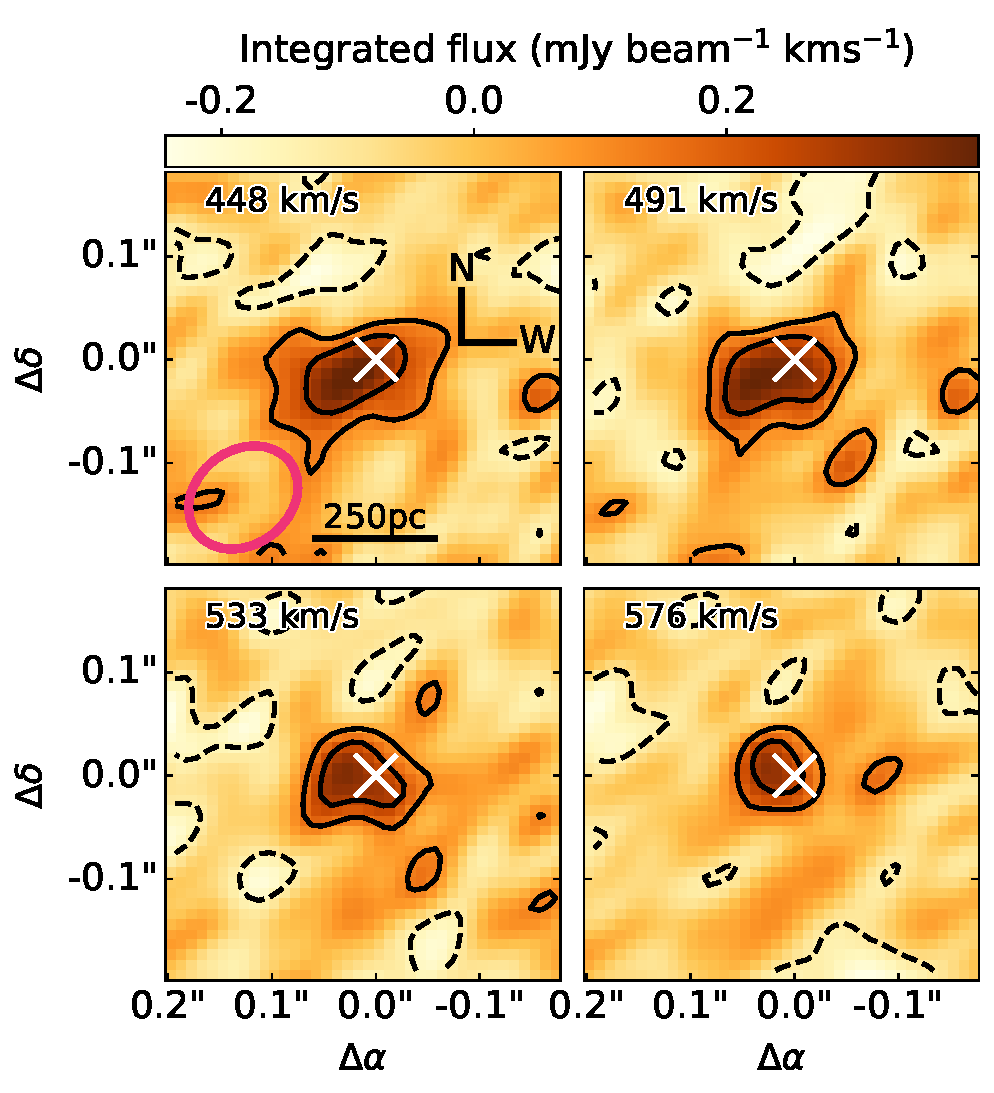
\includegraphics[width=0.75\linewidth]{figures/alma_f13451_1232/channel_maps.pdf}
    \caption[Velocity channel maps of the central $\sim$1\;kpc of the primary nucleus of F13451+1232.]{Channel maps of the central $\sim$1\;kpc of the primary nucleus of F13451+1232 (centred on the nucleus: Section\;\ref{section: alma_f13451_1232: observations_and_data_reduction}) between 448\;\textless\;$v$\;\textless\;576\;km\;s$^{-1}$, taken from the velocity-binned and smoothed cube with channel widths of 43.7\;km\;s$^{-1}$ and a velocity resolution of 86.4\;km\;s$^{-1}$. Black contours are shown at the $-3\sigma_\mathrm{rms}$, $-1.5\sigma_\mathrm{rms}$, 1.5$\sigma_\mathrm{rms}$, 3$\sigma_\mathrm{rms}$ levels (dashed: negative; solid: positive), where $\sigma_\mathrm{rms}$ is the RMS of the binned-and-smoothed cube. The continuum centre is marked as a white cross in each channel; the beam size is shown as a pink ellipse in the 448\;km\;s$^{-1}$ channel map (top left panel).}
    \label{fig: alma_f13451_1232: channel_maps}
\end{figure}

\vspace*{\fill}
\newpage

\subsection{Potential effects of continuum subtraction}
\label{section: alma_f13451_1232: analysis_and_results: potential_effects_of_continuum_subtraction}

Due to the bright, steep-spectrum continuum around the CO(1--0) line --- originating from primary nucleus of F13451+1232 (as seen in the cores of other CSS/GPS sources, e.g. \citealt{Oosterloo2019}) --- it is possible that inaccuracies in the continuum subtraction process have contributed flux to the compact, redshifted, high-velocity feature that is detected at the position of the nucleus. However, I argue that this feature represents real CO(1--0) emission, for several reasons. Firstly, the flux is detected above the $6\sigma$ level in the flux map integrated over the velocity range 400\;\textless\;$v$\;\textless\;680\;km\;s$^{-1}$ (Figure\;\ref{fig: alma_f13451_1232: outflow_moment_map}a), and in multiple velocity channels at the 3--4$\sigma_\mathrm{rms}$ levels (Figure\;\ref{fig: alma_f13451_1232: channel_maps}). Secondly, it has a significantly higher flux than the negative or positive residual features detected in the integrated spectrum (Figure\;\ref{fig: alma_f13451_1232: outflow_moment_map}b). 

Moreover, in Figure\;\ref{fig: alma_f13451_1232: beam_comparison}, I present CO(1--0) line spectra extracted from the two cubes of differing spatial resolution that comprise the combined datacube (Section\;\ref{section: alma_f13451_1232: observations_and_data_reduction}); the size of the extraction aperture in each case was matched to the beam size. The high-velocity redshifted feature is well detected in both datacubes in the velocity range 400\;\textless\;$v$\;\textless\;680\;km\;s$^{-1}$, while any residual features of comparable flux are not present in both cubes at the same velocity. Furthermore, its absolute flux is less in the smaller-beam cube, indicating that the beam is not recovering all of the flux and thus implying that the feature is (partially) spatially resolved. While some contribution from instrumental effects cannot be entirely ruled out, based on these arguments, I conclude that this feature is real.


\begin{figure}[!b]
    \centering
    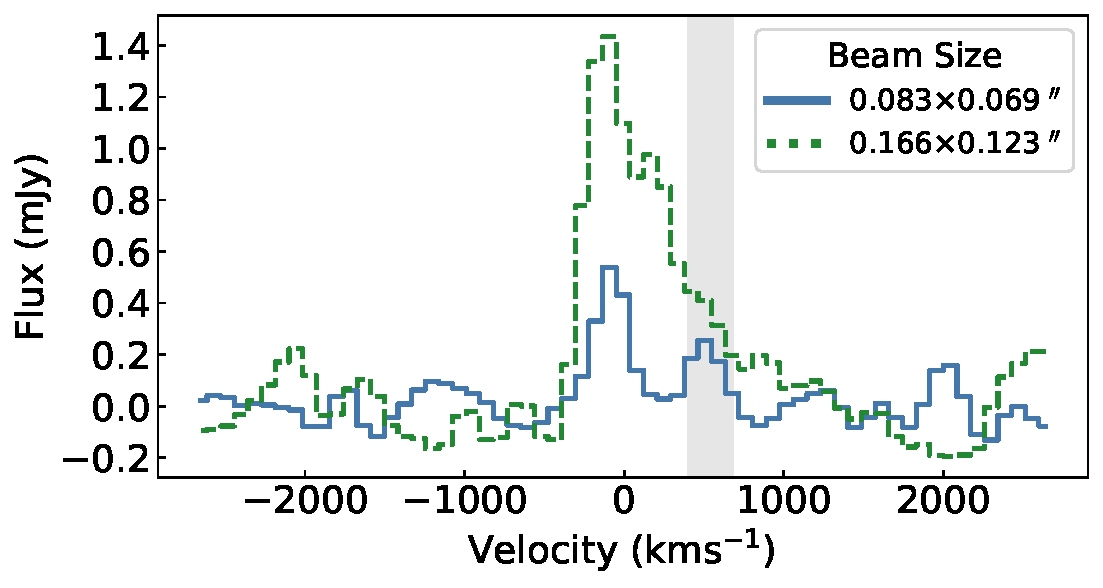
\includegraphics[width=0.75\linewidth]{figures/alma_f13451_1232/beam_comparison.pdf}
    \caption[CO(1--0) velocity profiles of the nuclear outflow in the primary nucleus of F13451+1232 extracted from observations of differing array configurations (hence beam sizes).]{CO(1--0) line profiles of the primary nucleus of F13451+1232 extracted from the two sets of observations of differing array configurations (hence beam sizes) that comprise the datacube presented in this analysis (see Section\;\ref{section: alma_f13451_1232: observations_and_data_reduction}). These profiles were extracted from the respective cubes using apertures matched to the beam sizes. It can be seen that the flux in the high-velocity redshifted component (shaded in grey) is less in the cube with the smaller beam size.}
    \label{fig: alma_f13451_1232: beam_comparison}
\end{figure}

It is notable that previous CO(2--1) observations of the primary nucleus of F13451+1232 --- that were of similar sensitivity to the CO(1--0) observations presented here --- did not detect evidence for nuclear outflows \citep{Lamperti2022}. However, in those observations, the other spectral windows were also used when fitting a linear slope to the continuum because of the narrower observing band (a factor of two narrower in velocity) of CO(2--1) observations relative to CO(1--0) --- this may have led to over-subtraction of the high-velocity outflow component. Therefore, it is possible that outflow emission in CO(2--1) was not detected due to uncertainties in the continuum subtraction process.

\subsection{Outflow energetics}
\label{section: alma_f13451_1232: analysis_and_results: outflow_energetics}

In order to provide an estimate of the mass inflow/outflow rates of the high-velocity, spatially-unresolved redshifted feature located at the position of the nucleus, an elliptical aperture matching the beam size ($0.113\times0.091$\;arcsec, PA$=-51.8^\circ$; shown in Figure\;\ref{fig: alma_f13451_1232: outflow_moment_map}a) was extracted from the datacube. I then summed all pixels within the aperture to create a line profile, which is presented in Figure\;\ref{fig: alma_f13451_1232: outflow_moment_map}b, and selected emission between 400\;\textless\;$v$\;\textless\;680\;km\;s$^{-1}$ to isolate the non-rotating gas. 

For the extended, intermediate-velocity (300\;\textless\;$|v|$\;\textless\;400\;km\;s$^{-1}$) emission seen in blueshift and redshift, two sub-apertures were extracted from the $1.00\times0.05$\;arcsecond slice along $\mathrm{PA}=120^\circ$ (used to create the upper PV diagram in Figure\;\ref{fig: alma_f13451_1232: pv_diagrams}): one covering radii 0.0\;\textless\;$r$\;\textless\;0.2\;arcseconds (for the extended redshifted emission), and the other covering the range 0.1\;\textless\;$r$\;\textless\;0.3\;arcseconds (for the extended blueshifted emission). I then selected emission in the ranges 300\;\textless\;$v$\;\textless\;400\;km\;s$^{-1}$ and $-400$\;\textless\;$v$\;\textless$-300$\;km\;s$^{-1}$ respectively in these slices to isolate the non-rotating gas.

For every channel within the range of the selected velocities in the extracted apertures, CO(1--0) fluxes ($S_\mathrm{CO}\Delta V$) were calculated and converted to luminosities ($L^\prime_\mathrm{CO}$) using the relation presented by \citet{Solomon2005}:
\begin{equation}
    L^\prime_\mathrm{CO} = 3.25\times10^7 S_\mathrm{CO}\Delta V {\nu}^{-2}_\mathrm{obs}D^2_\mathrm{L}(1+z)^{-3},
    \label{eq: alma_f13451_1232: co_luminosity}
\end{equation}
where ${\nu}_\mathrm{obs}$ is the observed frequency of the CO(1--0) line (102.789\;GHz) and $D_\mathrm{L}$ is the luminosity distance to F13451+1232. The CO(1--0) luminosities were then summed across all selected velocity channels, resulting in total luminosities for each of the two intermediate-velocity features and the high-velocity feature. Assuming a CO-to-H$_\mathrm{2}$ conversion factor of $\alpha_\mathrm{CO}=0.8$\;M$_\odot$\;(K\;km\;s$^{-1}$\;pc$^2$)$^{-1}$ (typical for ULIRGs: \citealt{Downes1998}), these total luminosities were converted into molecular gas masses ($M_\mathrm{flow}$). 

By taking an aperture covering the disk in the combined CO(1--0) datacube and integrating between $-310$\;\textless\;$v$\;\textless\;$310$\;km\;s$^{-1}$, a disk mass of $1.1\times10^{10}$\;M$_\odot$ was found using Equation \ref{eq: alma_f13451_1232: co_luminosity} and $\alpha_\mathrm{CO}=0.8$\;M$_\odot$\;(K\;km\;s$^{-1}$\;pc$^2$)$^{-1}$; \citet{Lamperti2022} also detected this nuclear disk using CO(2-1) spectroastrometry, and found a similar mass.

The corresponding mass flow rates of the non-rotating molecular gas were estimated using
\begin{equation}
    \dot{M}_\mathrm{flow} = \frac{M_\mathrm{flow}v_w}{\Delta R} \cdot \mathrm{tan\theta},
\end{equation}
where $v_w$ is the flux-weighted velocity, $\Delta R$ is the range of flow radii, and $\theta$ is the angle of the flow relative to the observer's line of sight. The $\mathrm{tan\theta}$ term is required to correct for projection effects in both radius and velocity. To estimate this projection factor, I assumed a solid-angle-weighted mean inclination for random orientations of the line of sight to the flow direction, giving $\theta=57.3^\circ$ \textbf{(see \citealt{Law2009} for a full derivation)}. Finally, kinetic powers were estimated with
\begin{equation}
    \dot{E}_\mathrm{kin}=\frac{1}{2}\dot{M}_\mathrm{flow}\Bigl(\frac{v_w}{\mathrm{cos\theta}}\Bigl)^2.
    \label{eq: alma_f13451_1232: kinetic_power}
\end{equation}
The resulting CO(1--0) luminosities, masses, flux-weighted velocities, flow radii, mass flow rates, kinetic powers, and coupling efficiencies ($\epsilon_\mathrm{f}=\dot{E}_\mathrm{kin}$/$L_\mathrm{bol}$) are given in Table\;\ref{tab: outflow_properties}. For the high-velocity nuclear gas, I derived a mass flow rate of $\dot{M}_\mathrm{out}\sim230$\;M$_\odot$\;yr$^{-1}$, which corresponds to a kinetic power that is $\sim$1.4\;per\;cent of the bolometric luminosity of the AGN ($L_\mathrm{bol}=4.8\times10^{45}$\;erg\;s$^{-1}$: \citealt{Rose2018}). In contrast, much lower mass flow rates ($\dot{M}_\mathrm{out}=22$--$27$\;M$_\odot$\;yr$^{-1}$) and kinetic powers ((6.0--7.1)$\times10^{-2}$\;per\;cent of $L_\mathrm{bol}$) were found for the extended, intermediate-velocity emission.

\begin{table*}[!t]
    \centering
    \renewcommand{\arraystretch}{1.1}
    \begin{tabular}{lcccc}
        \multirow{2}{*}{Component} & $L^\prime_\mathrm{CO}$  & $M_\mathrm{flow}$  & $v_\mathrm{w}$  & ${\Delta}R$ $^a$ \\
          & [K\;km\;s$^{-1}$\;pc$^{2}$] & [M$_\odot$] & [km\;s$^{-1}$] & [arcsec] \\
        \hline
        Extended blueshifted & $2.7\times10^7$ &  $2.2\times10^7$  & $-339$ & 0.2  \\
        Extended redshifted &  $2.2\times10^7$  & $1.8\times10^7$ & 350 & 0.2 \\
        Nuclear redshifted & $4.2\times10^7$ & $3.4\times10^7$ & 514 & 0.0545
    \end{tabular} \\
    \vspace*{12pt}
    \centering
    \begin{tabular}{lcccc}
        \multirow{2}{*}{Component} & $\dot{M}_\mathrm{flow, proj}$ & $\dot{M}_\mathrm{flow}$  & $\dot{E}_\mathrm{kin}$  & $\epsilon_\mathrm{f}$ $^b$ \\
          &  [M$_\odot$\;yr$^{-1}$] & [M$_\odot$\;yr$^{-1}$] & [erg\;s$^{-1}$] & [per\;cent] \\
        \hline
        Extended blueshifted & 17 & 27 & $3.4\times10^{42}$ & $7.1\times10^{-2 }$  \\
        Extended redshifted & 14 & 22 &  $2.9\times10^{42}$ & $6.0\times10^{-2}$ \\
        Nuclear redshifted & 148 & 230 & $6.6\times10^{43}$ & 1.4
    \end{tabular}
    \vspace*{12pt} \\
    \centering
    $^a$For the extended emission, ${\Delta}R$ is taken to be the radial distance over which the extended emission is seen; for the spatially-unresolved, high-velocity redshift feature, ${\Delta}R$ is taken to be half of the beam major axis. \\
    $^b$Calculated assuming $L_\mathrm{bol}=4.8\times10^{45}$\;erg\;s$^{-1}$ \citep{Rose2018}.
    \caption[CO(1--0) luminosities, masses, projected flux-weighted outflow velocities, aperture radii, projected mass flow rates ($\dot{M}_\mathrm{flow, proj}$), deprojected mass flow rates ($\dot{M}_\mathrm{flow}$), and deprojected energetics for the molecular gas components in the primary nucleus of F13451+1232, including for the compact nuclear outflow.]{CO(1--0) luminosities, masses, projected flux-weighted flow velocities, aperture radii, projected mass flow rates ($\dot{M}_\mathrm{flow, proj}$), deprojected mass flow rates ($\dot{M}_\mathrm{flow}$), and deprojected energetics for the extended emission in both blueshift and redshift, and the nuclear redshifted feature seen in the PV diagrams (Figure\;\ref{fig: alma_f13451_1232: pv_diagrams}). When deprojecting, $\theta=57.3^\circ$ was assumed.}
    \label{tab: outflow_properties}
\end{table*}


\section{Discussion}
\label{section: alma_f13451_1232: discussion}

In addition to a kpc-scale disk, this analysis has detected non-rotating cold-molecular gas in CO(1--0) emission near the primary nucleus of F13451+1232. This non-rotating gas consists of spatially-extended (0.0\;\textless\;$r$\;\textless\;0.3\;arcseconds; 0\;\textless\;$r$\;\textless\;660\;pc), intermediate-velocity (300\;\textless\;$|v|$\;\textless\;400\;km\;s$^{-1}$) components seen in both blueshift and redshift, and a compact ($r$\;\textless\;0.06\;arcseconds; $r$\;\textless\;120\;pc), high-velocity (400\;\textless\;$v$\;\textless\;680\;km\;s$^{-1}$) nuclear component seen in redshift.

\subsection{Interpreting the non-rotating gas as inflowing}
\label{section: alma_f13451_1232: discussion: inflows}

Given that the AGN in F13451+1232 may have recently restarted and thus be young \citep{Stanghellini2005, Morganti2013_4c1250}, if the non-rotating gas seen in intermediate and high-velocity CO(1--0) emission is inflowing, it is possible that it represents gas flows responsible for its triggering. The total gas flow rates (22--230\;M$_\odot$\;yr$^{-1}$: Table\;\ref{tab: outflow_properties}) are orders of magnitude higher than those needed to sustain the AGN (0.8\;M$_\odot$yr$^{-1}$, assuming $\eta=0.1$ and $L_\mathrm{bol}=4.8\times10^{45}$\;erg\;s$^{-1}$: \citealt{Rose2018}). Therefore, this is a plausible feeding mechanism even if only a small fraction of the inflowing gas is accreted onto the central supermassive black hole. However, I argue later that the compact, high-velocity component (and potentially also the intermediate-velocity emission) is in reality outflowing, rather than inflowing.

\subsection{The spatially-extended, intermediate-velocity gas}
\label{section: alma_f13451_1232: discussion: intermediate_velocity_gas}

The nature of the intermediate-velocity emission (300\;\textless\;$|v|$\;\textless\;400\;km\;s$^{-1}$) that is seen in both redshift and blueshift in the PV diagram along $\mathrm{PA}=120^\circ$ (Figure\;\ref{fig: alma_f13451_1232: pv_diagrams}) --- and as a region of higher velocity dispersion to the SE of the nucleus in the moment 2 maps (Figure \ref{fig: alma_f13451_1232: moment_maps}) --- is not clear. On one hand, it may represent spatially-extended (220\;\textless\;$r$\;\textless\;440\;pc) AGN-driven outflows. However, since the emission extends well beyond the compact radio source, then these outflows would not be driven solely by the jet --- an additional outflow driving mechanism would be required. Based on the similar PAs of the extended emission and the small-scale radio structure, one possibility is that this gas is accelerated by radiatively-driven winds that are collimated by a circumnuclear torus with an axis similar to that of the compact radio source.  Alternatively, due to the velocities not being much above those expected for rotation (as given by the \textsc{BBarolo} model: Section\;\ref{section: alma_f13451_1232: analysis_and_results: disk}), this extended emission may represent material from the merger settling onto the disk. This latter interpretation is supported by the larger-scale ($r$\;\textgreater\;1\;kpc) filament-like structures seen to the south and west of the primary nucleus (Figure\;\ref{fig: alma_f13451_1232: moment_maps}), which likely represent gas disturbed by the merger: these large-scale structures have similar velocity shifts and dispersions to the intermediate-velocity gas seen near the nucleus.

If the intermediate-velocity emission truly did represent AGN-driven outflows, then its mass outflow rates (22--27\;M$_\odot$\;yr$^{-1}$) are higher than those of the previously detected warm ionised (11.3\;M$_\odot$\;yr$^{-1}$: \citealt{Rose2018})\footnote{The warm-ionised mass outflow rates and kinetic powers were calculated following the second method of \citet{Rose2018}, which involves using the $v_\mathrm{05}$ parameter as the outflow velocity to account for projection effects; these estimates are likely to be upper limits.} and neutral HI ($\sim$6\;$M_\odot$\;yr$^{-1}$)\footnote{The neutral HI mass outflow rate has been recalculated using the methodology in Section\;\ref{section: xshooter_ic5063: discussion: multiphase: energetics} with the values presented by \citet{Morganti2013_4c1250}; the kinetic power and coupling efficiency have been recalculated by using these values with Equation \ref{eq: alma_f13451_1232: kinetic_power} and assuming $L_\mathrm{bol}=4.8\times10^{45}$\;erg\;s$^{-1}$ \citep{Rose2018}.} phases. Furthermore, they are similar to those recently reported for the cold-molecular outflows in a sample of nearby QSO2s (8--16\;M$_\odot$\;yr$^{-1}$: \citealt{RamosAlmeida2022}), which were identified using a similar method to that used here for the intermediate-velocity gas. When applying a factor of three to account for assumed outflow geometry, as was done by \citet{Fiore2017}, I find (in agreement with \citealt{RamosAlmeida2022}) that these mass outflow rates (66--81\;M$_\odot$\;yr$^{-1}$) fall significantly below the correlation between mass outflow rate and AGN bolometric luminosity given by \citet{Fiore2017} (Figure\;\ref{fig: introduction: outflows: acceleration_mechanisms: fiore2017_mout_ekin_lbol}). However, it is important to note that \citet{Lamperti2022} reported a wide range of mass outflow rates for ULIRGs with similar bolometric luminosities (6\;\textless\;$\dot{M}_\mathrm{flow}$\;\textless\;300\;M$_\odot$\;yr$^{-1}$), indicating that the high mass outflow rates found by \citet{Fiore2017} may represent the most extreme cases, and therefore represent the upper envelope to any relationship between mass outflow rate and AGN bolometric luminosity (see also \citealt{Speranza2024}).

\subsection{The compact, high-velocity nuclear outflow}
\label{section: alma_f13451_1232: discussion: nuclear_outflow}

While it is possible that the intermediate-velocity emission does not represent outflowing gas, I highlight that the observed velocities of the redshifted nuclear feature (400\;\textless\;$v$\;\textless\;680\;km\;s$^{-1}$) are much higher than what would be expected due to settled gravitational motions ($v$\;\textless\;300\;km\;s$^{-1}$: the projected velocities seen in the disk). Moreover, the emission of this component is compact ($r$\;\textless\;120\;pc), unresolved in the combined datacube, and on a similar radial scale to both the compact radio structure ($r$\;\textless\;0.06\;arcseconds; $r$\;\textless\;130\;pc: Figure\;\ref{fig: alma_f13451_1232: outflow_moment_map}a) and the other outflow phases ($r$\;\textless\;100\;pc: \citealt{Morganti2013_4c1250, Tadhunter2018}). Therefore, it is much more likely to be a nuclear outflow, rather than an inflow or settling gas from the merger. Furthermore, the fact that the high-velocity emission is spatially offset from the nucleus \textbf{(by $32\pm2$\;milliarcseconds)} along the direction of the small-scale radio structure ($\mathrm{PA}=151^\circ$) suggests a relation between the two. This is consistent with acceleration by shocks, which may be induced by either a jet or a broader, radiatively-driven wind that is collimated by the circumnuclear torus. Given that the compact CO(1--0) outflow is seen to be offset along the direction of the radio structure (which would not necessarily be expected in the radiatively-driven scenario), and that the neutral-atomic outflow component (detected in HI absorption) is seen to be coincident with the radio hotspot \citep{Morganti2013_4c1250}, I favour the jet-driven interpretation. In this context, it is interesting to note the southern bend in the small-scale radio structure, which may be due to the jet colliding with dense molecular gas, being deflected, and thereby launching the nuclear outflow.

The fact that this nuclear outflow is partially spatially resolved by the smaller-beam observations (Figure \ref{fig: alma_f13451_1232: beam_comparison}) allows the outflow radius to be constrained to be in the range 88\;\textless\;$\Delta{R}$\;\textless\;182\;pc (0.042\;\textless\;$\Delta{R}$\;\textless\;0.083\;arcseconds; i.e. half of the beam major axes of the two constituent observations: Section\;\ref{section: alma_f13451_1232: observations_and_data_reduction}). Considering that the feature does not appear to be spatially resolved in the channel maps (Section\;\ref{section: alma_f13451_1232: analysis_and_results: channel_maps}; Figure\;\ref{fig: alma_f13451_1232: channel_maps}) produced from the combined datacube (beam size: $0.113\times0.091$\;arcseconds; see Section\;\ref{section: alma_f13451_1232: observations_and_data_reduction}), this indicates that it is, overall, partially spatially resolved in the ALMA CO(1--0) observations --- I thus take 120\;pc (0.0545\;arcseconds) as an upper limit on the outflow radius.

The cold-molecular mass outflow rate for this nuclear component ($\dot{M}_\mathrm{flow}\sim230$\;M$_\odot$\;yr$^{-1}$) is more than an order of magnitude higher than those previously derived for the other outflow phases in F13451+1232, lies within the range of values for molecular outflows previously detected in ULIRGs (a few to thousands of solar masses per year: \citealt{Cicone2014, Pereira-Santaella2018, Fluetsch2019, Herrera-Camus2020, Lamperti2022}), and is close to (within 1$\sigma$ of) the correlation between cold-molecular mass outflow rate and AGN bolometric luminosity found by \citet{Fiore2017} when corrected for assumed outflow geometry.

Overall, the kinetic power of the cold molecular phase in F13451+1232 ($6.6\times10^{43}$\;ergs$^{-1}$) accounts for $\sim$1.4\;per\;cent of $L_\mathrm{bol}$ --- approximately a factor of three higher than the combined kinetic power of the neutral HI ($\sim$0.04\;per\;cent of $L_\mathrm{bol}$: \citealt{Morganti2013_4c1250}) and warm ionised (0.49\;per\;cent of $L_\mathrm{bol}$: \citealt{Rose2018}) outflow phases. Therefore, for all phases, the \textit{total} outflow kinetic power is $\sim$2\;per\;cent of the AGN bolometric luminosity. While this is consistent with the requirements of simulations of outflows launched by AGN in galaxy mergers (0.5\;\textless\;$\epsilon_\mathrm{f}$\;\textless\;10\;per\;cent: e.g. \citealt{DiMatteo2005, Hopkins2010}) --- and thus may be interpreted as the outflows having an impact on the evolution of the galaxy --- I highlight that such comparisons must be done with care, and that it is unclear if interpretations can be made robustly (see Section\;\ref{section: introduction: outflows: comparisons_to_models} and \citealt{Harrison2018}).

Finally, I emphasize that even if a CO-to-H$_\mathrm{2}$ conversion factor that is at the lower end of the range of values used in the literature (i.e. $\alpha_\mathrm{CO}=0.3$\;M$_\odot$\;(K\;km\;s$^{-1}$\;pc$^2$)$^{-1}$ for optically thin gas: \citealt{Oosterloo2017, Oosterloo2019}) is assumed, the derived cold-molecular, nuclear mass outflow rate is still much higher than those of the other phases ($\sim$86\;M$_\odot$yr$^{-1}$). Conversely, if a conversion factor that is characteristic of molecular clouds in the Milky Way is assumed ($\alpha_\mathrm{CO}=4.3$\;M$_\odot$\;(K\;km\;s$^{-1}$\;pc$^2$)$^{-1}$: \citealt{Bolatto2013}), the mass and kinetic power of this outflow increase significantly ($\dot{M}_\mathrm{out}\sim1240$\;M$_\odot$\;yr$^{-1}$; $\epsilon_\mathrm{f}\sim7$\;per\;cent).

\section{Chapter conclusions}
\label{section: alma_f13451_1232: conclusions}

Through the analysis of high-spatial-resolution CO(1--0) observations of the primary nucleus of the ULIRG F13451+1232, this chapter has presented evidence for (and has characterised) a kpc-scale circumnuclear disk and spatially-extended (0.0\;\textless\;$r$\;\textless\;0.3\;arcseconds; 0\;\textless\;$r$\;\textless\;660\;pc), intermediate-velocity emission (300\;\textless\;$|v|$\;\textless\;400\;km\;s$^{-1}$). This intermediate-velocity molecular gas may represent AGN-radiation-driven outflows, or merger material settling onto the disk. Furthermore, I have presented evidence for a compact ($r$\;\textless\;120\;pc), jet-driven cold-molecular outflow (400\;\textless\;$v$\;\textless\;680\;km\;s$^{-1}$) at the position of the nucleus, with a mass outflow rate of $\dot{M}_\mathrm{out}\sim230$\;M$_\odot$\;yr$^{-1}$ and a kinetic power that is $\sim$1.4\;per\;cent of the AGN bolometric luminosity.

Overall, this detection of cold molecular outflow(s) in F13451+1232 changes the scenario of the AGN-driven outflows in the object: previous studies found that the neutral atomic HI and warm ionised phases had relatively modest mass outflow rates, whereas here it is found that the cold-molecular outflow is carrying over an order of magnitude more mass (and several times the kinetic power) than the warm ionised and neutral atomic phases. Similar results have been found for other types of active galaxy, where the colder phases have been seen to carry the majority of the outflowing mass \citep{RamosAlmeida2019, Speranza2024}, including IC\;5063 (Chapter \ref{chapter: xshooter_ic5063}) and NGC\;1068 (Chapter \ref{chapter: stis_seyferts}). This further demonstrates the need for multi-wavelength observations to fully quantify the impact of AGN-driven outflows. Moreover, a similarly compact ($r$\;\textless\;120\;pc) but more massive ($\dot{M}_\mathrm{out}\sim650$\;M$_\odot$\;yr$^{-1}$) outflow was found in the ULIRG PKS\;1549-79 \citep{Oosterloo2019}, which is also both a merger and a luminous radio source. These results thus provide important evidence that powerful radio sources accelerate compact molecular outflows, and that these outflows may carry more mass and power than other gas phases.

Crucially, in demonstrating that cold-molecular AGN-driven outflows can be compact ($r$\;\textless\;$120$\;pc), this chapter emphasises the importance of high-spatial-resolution observations when robustly quantifying the impact of AGN-driven outflows on their host galaxies.

\vspace*{\fill}

\section*{Chapter acknowledgements}
\addcontentsline{toc}{section}{\protect\numberline{}Chapter acknowledgements}

I thank the anonymous referee of the publication that this chapter is based on for their feedback, which helped to improve the quality of the report. This chapter makes use of the following ALMA data: ADS/JAO.ALMA\#2019.1.01757.S. ALMA is a partnership of ESO (representing its member states), NSF (USA) and NINS (Japan), together with NRC (Canada), MOST and ASIAA (Taiwan), and KASI (Republic of Korea), in cooperation with the Republic of Chile. The Joint ALMA Observatory is operated by ESO, AUI/NRAO and NAOJ. The European VLBI Network is a joint facility of independent European, African, Asian, and North American radio astronomy institutes. Scientific results from data presented in this publication are derived from the following EVN project code(s): GM062.

\section*{Data availability}
\addcontentsline{toc}{section}{\protect\numberline{}Data availability}

The ALMA CO(1--0) data used in this work is publicly available from the ALMA Science Archive (\url{https://almascience.eso.org/aq/}) with Project Code 2019.1.01757.S. The data used to produce the VLBI 1266\;MHz continuum image presented in Figure\;\ref{fig: alma_f13451_1232: outflow_moment_map}a is publicly available from the European VLBI Network archive for experiment GM062B (\url{http://archive.jive.nl/scripts/arch.php?exp=GM062B_060605}).
